\chapter{Overall Description}
\label{ch:overall}

\section{\jel{} System Structure}
\label{sec:structure}
\includegraphics[height=10cm]{communicationmodel.eps}
\section{\mcode{} functions}
\label{sec:functions}
\mcode{} is the intermediate language used to communicate the visualization engine and the Java interpreter (\djava{}). It mainly flows from \djava{}to the Director.  The information that carries along within is not only the information about modified variables and modified method stacks, but also the operations that produce such changes. and the results of those operations. This is the biggest difference from normal compiler intermediate codes; they only indicate what operations to perform to the assembler. In our case all operations are performed and the every result is sent to the Director.

\section{User Characteristics}
\label{sec:users}

This document is addressed to the following people:

\begin{description}
	\item[Developer of Visualization Systems] This document may provide ideas and solutions to developers of new visualization systems, as well as provides of an existing solution that can be merged into their ongoing projects.
	
	\item[Maintainer of \jel{}] Future developers and maintainers of \jel{} should refer to this document when modifying its source code, specially those files referring to \djava{} and \jel{}'s interpreter. They should incorporate here all changes done to \mcode{} to provide a state of the art document as well. 
	
\end{description}

\section{Features and Constraints}
\label{sec:features}

While trying to produce the more generic intermediate code some features and constraints where placed due to several reasons. The most important ones are the following ones:

\begin{description}
	\item[Java] Being Java the language of choice, \mcode{} supports most of its characteristics and abilities. It is object oriented, so things as method calls, objects and, to some extend, inheritance are supported.
	
	\item[\djava{}]Because of using \djava{} as an interpreter from which to extract the execution information, some of the specified ordered sequences of instructions may be too constrained to the particularity of \djava{}. However that is not the case for the most of instructions explained here.
	
	\item[Targeted audience] \mcode{} was designed to support the development of \mcode{}, thus it was important to address their specific problems: \mcode{} has a great detail in the evaluation of expressions and the normal flow of program, so novices will grasp the programming fundamental issues. Meanwhile, more advanced features are not within the scope of the \mcode{} and have not been implemented. Those features include threads, reflection utilities and exception handling. 
	
\end{description}

\section{Dependencies}
\label{sec:dependencies}

Right now \mcode{} is only produced through the modified version of \djava{} included in the distribution of \jel{}. However it is up to anyone to create a new high\-{}level interpreter to produce its own \mcode{} to be run by \jel{}'s \mcode{} interpreter or by one they develop. 
There is also the possibility to store the \mcode{} a single text file and be retrieved later by a \mcode{} interpreter to produce visualization orders. However, this configuration would not allow INPUT/OUTPUT operations as they provide information to the evaluation needed to carry on with following instructions. 